
\documentclass[11pt]{article} 
\usepackage{amsmath, amssymb}
\usepackage{graphicx}
\usepackage{hyperref}
\usepackage{cite}
\usepackage{float}
\usepackage{geometry}
\geometry{margin=1in}
\title{Real-Time Traffic Object Detection Using YOLOv5 with COCO-Based Transfer Learning for CPU Deployment}
\author{Jamal Bouheur \and Jason Nguyen \\
        CS4277 \\
        Kennesaw State University \\
        \texttt{jbonheur@students.kennesaw.edu,jnguy203@students.kennesaw.edu}}
\date{\today}

\begin{document}

\maketitle

\section{Abstraction}
Object detection is a critical component in autonomous driving and intelligent transportation systems. In this study, we propose a real-time traffic object detection framework using YOLOv5, targeting four key object categories: cars, traffic lights, traffic signs, and pedestrians. To enhance performance and reduce training time, we leverage transfer learning by initializing YOLOv5 with weights pre-trained on the COCO dataset. The model is then fine-tuned on a subset of the BDD100K dataset to adapt to diverse urban traffic scenarios, including variations in lighting, weather, and object density. Additionally, the model is optimized for inference on CPU-only environments, enabling real-time deployment on low-power or embedded devices without GPU acceleration. Experimental results demonstrate that the system achieves high detection accuracy and responsiveness, confirming the feasibility of using YOLOv5 with COCO-based transfer learning for efficient and scalable traffic scene understanding in resource-constrained settings.


\section{Introduction}
Deep learning has transformed computer vision, enabling accurate and efficient real-time object detection. In autonomous driving and intelligent transportation systems, detecting traffic-related objects such as cars, traffic lights, traffic signs, and pedestrians plays a key role in decision-making. YOLOv5 has become a popular choice for object detection due to its speed and accuracy, leveraging a single neural network to predict both bounding boxes and class probabilities simultaneously.

In this paper, we apply YOLOv5 for traffic object detection by fine-tuning it with transfer learning using pre-trained weights from the COCO dataset. This approach accelerates training and improves performance, particularly for objects less represented in the training data. We further fine-tune the model on the BDD100K dataset, which includes diverse urban traffic scenarios.

To ensure practical deployment, we optimize the model for CPU-only environments, making it suitable for real-time applications on edge devices. This combination of transfer learning and CPU optimization provides an efficient solution for real-time traffic scene understanding.
\section{Methodology}
The core methodology involves the application of YOLOv5, a state-of-the-art object detection model, which is initially pre-trained on the COCO dataset. This transfer learning approach allows the model to leverage previously learned features and accelerate the training process, particularly for objects not widely represented in the training data. YOLOv5 is then fine-tuned on the BDD100K dataset, which contains diverse traffic scenarios, enabling the model to recognize and classify objects under varying conditions, such as lighting, weather, and traffic density.

We used the BDD100K dataset, a large-scale driving video dataset, for training our YOLOv5 model. From the dataset, we selected 10,000 images, allocating 7,000 for training and 3,000 for validation. Our task focused on detecting four classes of traffic-related objects: car, traffic sign, traffic light, and pedestrian. The annotations were converted into YOLO format, and images were resized to 640×640 resolution for consistency. Training was conducted on a T4 GPU using the Adam optimizer with a learning rate of 0.01. We trained the model for 200 epochs with a batch size of 16. These hyperparameters were chosen to balance model convergence and training efficiency.  Illustrate the instance of classes distribution in figure. 
\begin{figure}[H]
    \centering
    \includegraphics[width=0.8\textwidth]{/Users/jasonnguyen/Downloads/yes.jpg}
    \caption{Distribution of object instances per class (cars, traffic lights, signs, and pedestrians)}
    \label{fig: class distribution}
\end{figure}

To optimize for CPU-only environments, the model is fine-tuned and optimized to reduce the computational overhead while maintaining real-time inference performance. This is particularly important for deployment in systems with limited resources, such as traffic cameras, embedded systems, and real-time surveillance platforms.

\section{Results}


\subsection{Object Detection Examples}
\begin{figure}[H]
    \centering
    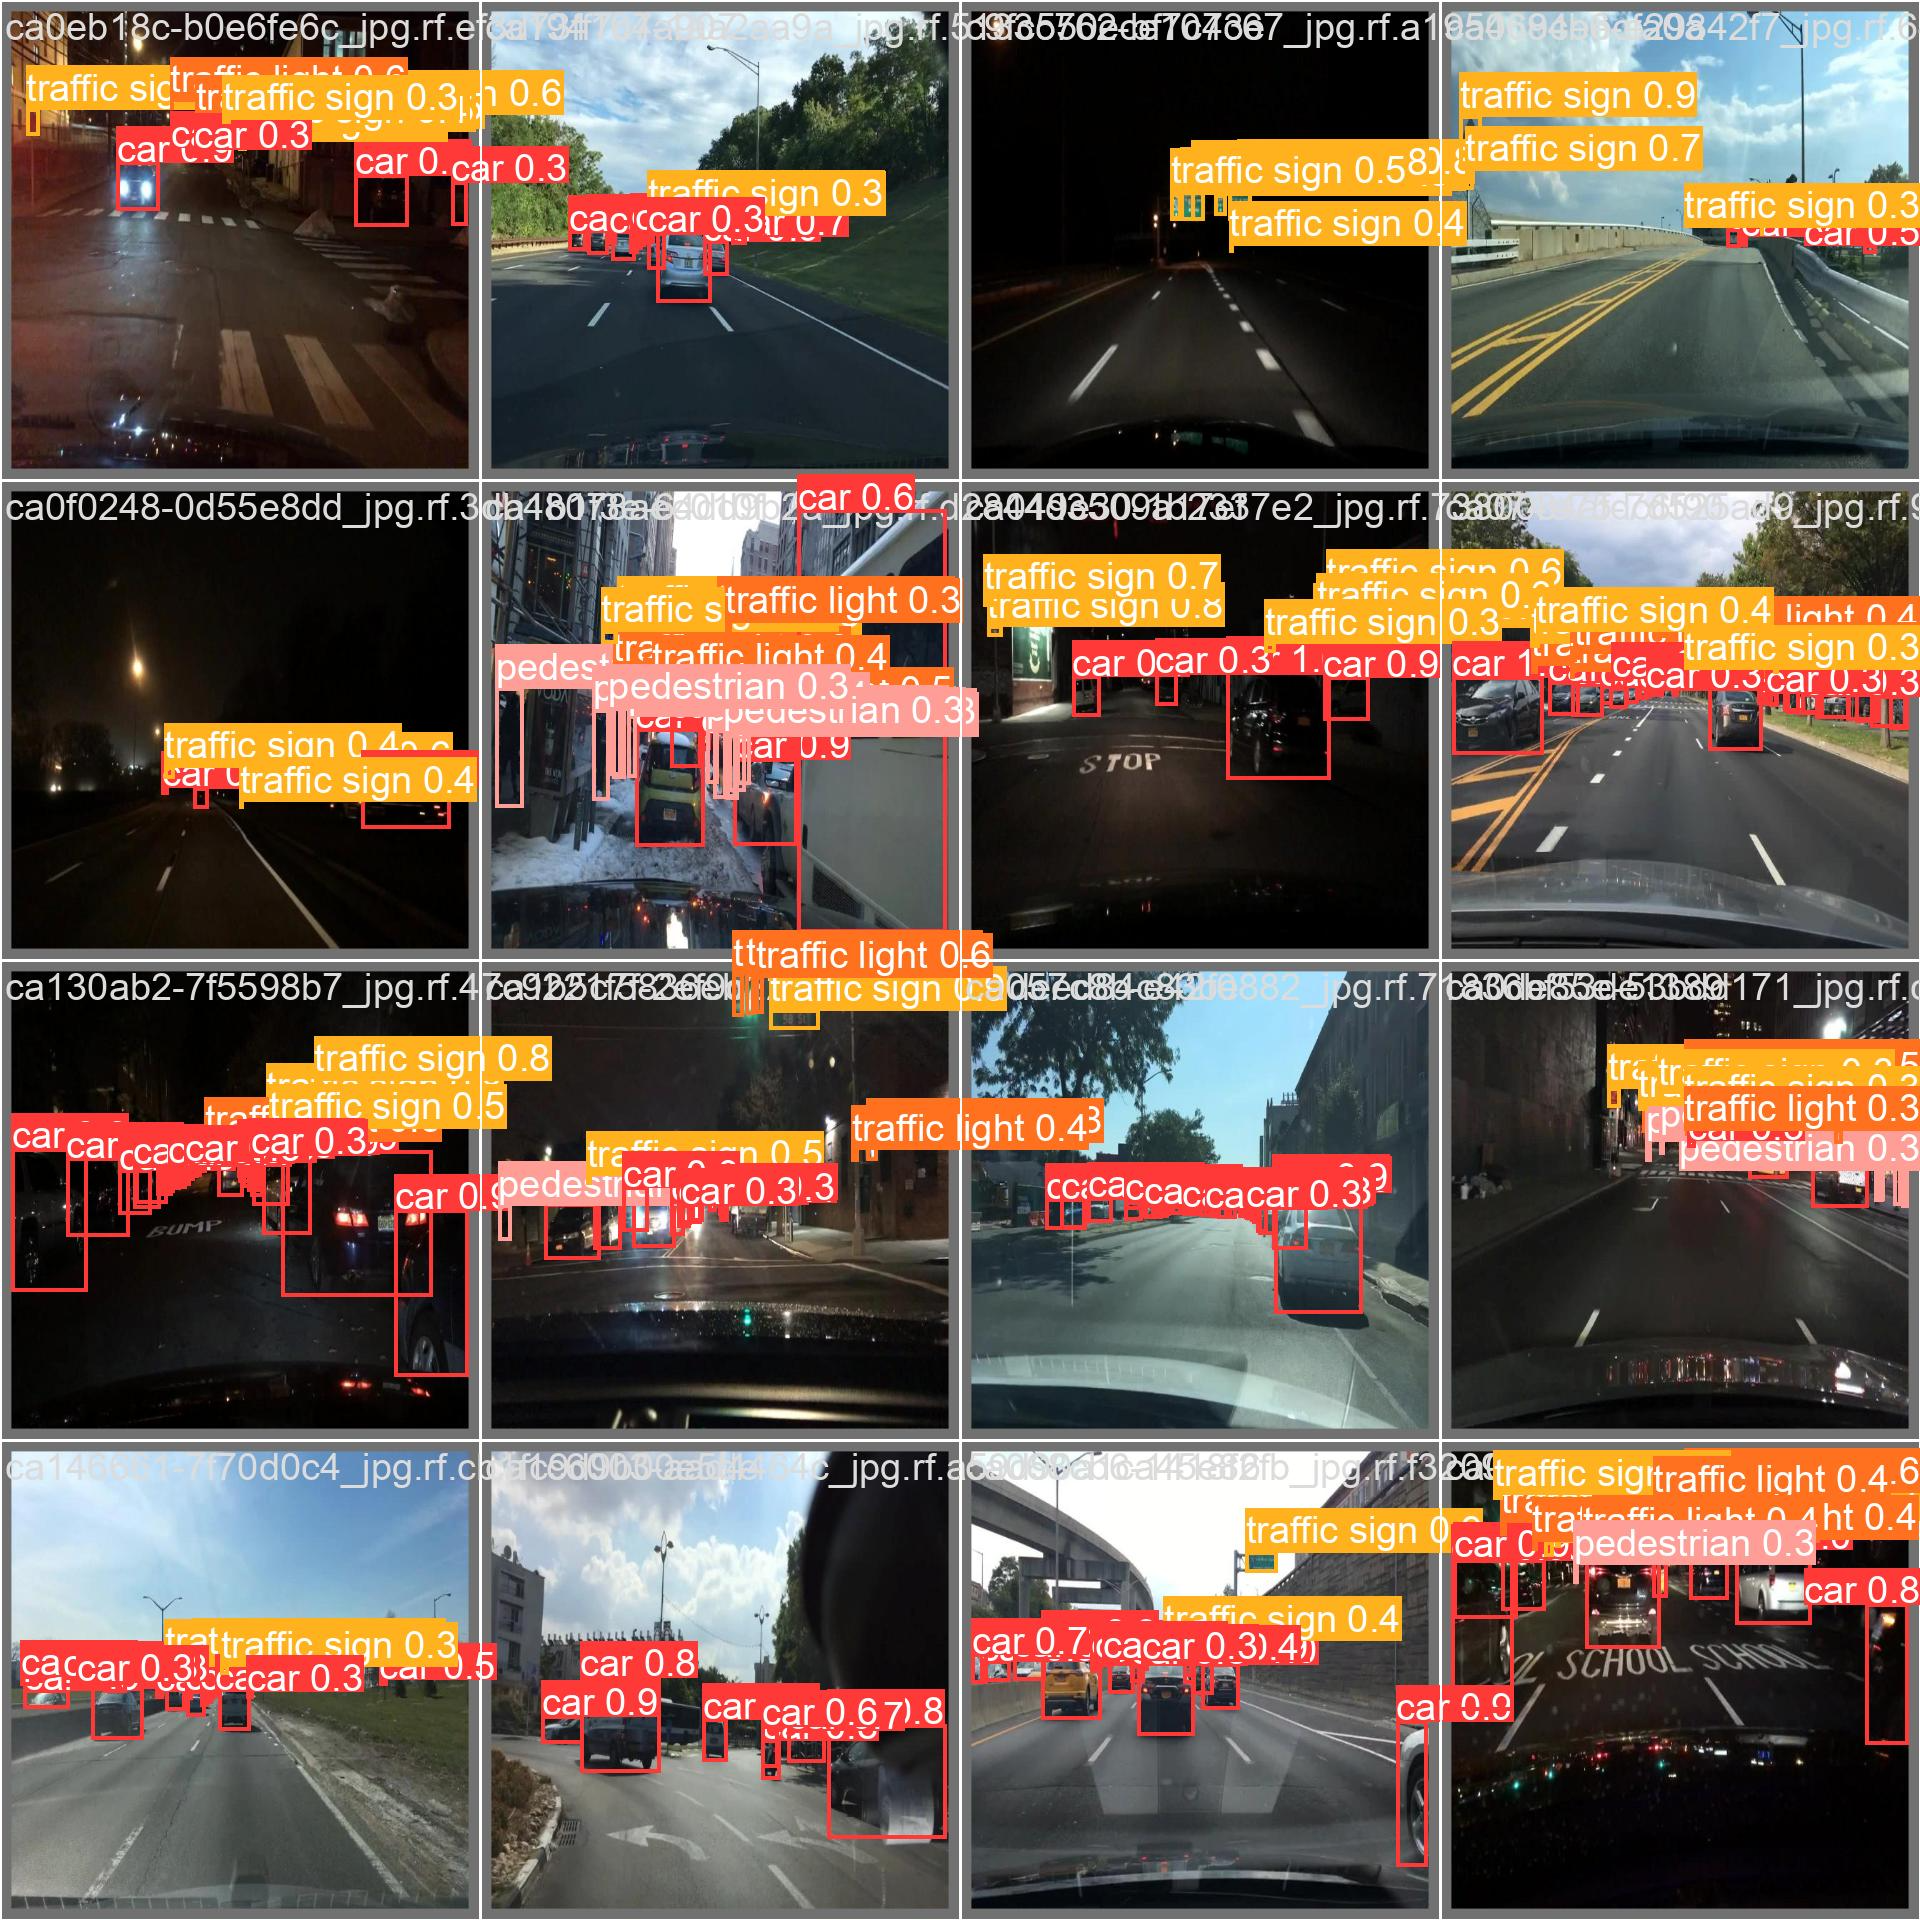
\includegraphics[width=0.8\textwidth]{/Users/jasonnguyen/Downloads/media_images_Validation_200_334cb4e652358e67d8ad.jpg}
    \caption{Sample images with detected objects (cars, traffic lights, signs, and pedestrians) using YOLOv5. Bounding boxes and class labels are shown for each detected object.}
    \label{fig:detection_example_1}
\end{figure}
\subsection{Model Performance Metrics}

\begin{figure}[H]
    \centering
        \includegraphics[width=0.8\textwidth]{/Users/jasonnguyen/Downloads/CS4277_ResearchPaper/media_images_Results_200_3bf03f513a8b95dcd398.png}
    	\includegraphics[width=0.8\textwidth]{/Users/jasonnguyen/Downloads/CS4277_ResearchPaper/media_images_Results_200_c3835e97ccb97e8b4e52.png}

        \caption{Precision, Recall, and F1-score for YOLOv5 object detection across different categories.}
    \label{fig:metrics}
\end{figure}

\subsection{Inference Time}
\begin{figure}[H]
    \centering
    \includegraphics[width=0.8\textwidth]{/Users/jasonnguyen/Downloads/frame.png}

    \caption{FPS for YOLOv5 in detecting various traffic objects on CPU.}
    \label{fig:fps}
\end{figure}

\subsection{Confusion Matrix}
\begin{figure}[H]
    \centering
     \includegraphics[width=0.8\textwidth]{/Users/jasonnguyen/Downloads/CS4277_ResearchPaper/media_images_Results_200_ed3ee67b4f2f578c66f9.png}
    \caption{Confusion matrix for YOLOv5 detection performance across different traffic object categories.}
    \label{fig:confusion_matrix}
\end{figure}


\section{Conclusion}
This research paper has demonstrated the potential of YOLOv5 for traffic object detection with a focus on transfer learning from the COCO dataset and CPU-based deployment. The findings show that YOLOv5 can achieve significant performance in real-time object detection, balancing inference time and accuracy. The experiments conducted have provided a valuable analysis of the model's capability in a traffic environment and its suitability for practical deployment. Several challenges and areas for improvement have been identified in this study. First, future research should consider using more varied datasets, encompassing a wider range of traffic conditions, to assess the model's generalizability and performance under different environmental factors. Second, while the trade-off between inference time and accuracy was explored, additional methods for improving both performance metrics could be investigated. Ensuring that a model is both fast and accurate in traffic object detection remains a critical challenge. Third, real-world testing in diverse traffic environments is essential to provide a clearer understanding of how well these models perform outside controlled settings. Finally, the deployment of these models on different hardware platforms, such as edge devices, GPUs, and CPUs, can impact inference time significantly. Future studies should explore the interaction between model choice and hardware for optimal performance. These future improvements in traffic object detection can enhance both the practical applications of these systems and the real-time processing requirements necessary for deployment in everyday traffic scenarios.


\bibliographystyle{plain}  
\begin{thebibliography}{9}

\bibitem{yu2020bdd100k}
F. Yu, H. Chen, X. Wang, W. Xian, Y. Chen, F. Liu, V. Madhavan, and T. Darrell, 
``BDD100K: A Diverse Driving Dataset for Heterogeneous Multitask Learning,'' 
\textit{Proceedings of the IEEE/CVF Conference on Computer Vision and Pattern Recognition (CVPR)}, 
pp. 2636--2645, 2020.
\bibitem{yolov5}
Glenn Jocher, 
``YOLOv5: A state-of-the-art object detection model,''
\url{https://github.com/ultralytics/yolov5}, 
Accessed: 2025-04-30.

\end{thebibliography}

\end{document}

